\chapter{Curvas intensidad--potencial}\label{ch:b2:current-potential-curves}

El cinc se deposita electrolíticamente sobre el acero a partir de baños ácidos. Sin embargo, el diagrama E--pH del
volumen del primer año dice que el cinc, muy por debajo de la recta del hidrógeno, debería reducir
el ácido y disolverse tan deprisa como se deposita. No lo hace, porque un
diagrama dice lo que puede ocurrir, no a qué velocidad. La velocidad de una reacción de electrodo
es una corriente, y representar esa corriente en función del potencial del electrodo
muestra de inmediato qué reacciones son rápidas, cuáles son lentas y cuáles están frenadas
por el aporte de reactivo. Estas \omterm{def:b2:current-potential-curves:ie-curve}{curvas intensidad--potencial} son la herramienta
de todo electroquímico que recubre un metal, carga una batería o mide el
oxígeno de un río.

\begin{recall}
El volumen del primer año: potencial de electrodo, electrodo de referencia, la ecuación
de Nernst, los diagramas E--pH y su límite (dicen lo que es posible, no a qué
velocidad). \Cref{ch:b2:cell-thermodynamics}: $\Delta_r G = -nFE$, la ecuación de
Nernst deducida. De la física: la difusión y la ley de Fick, $j = -D\,dc/dx$.
\end{recall}

\begin{omfigure}
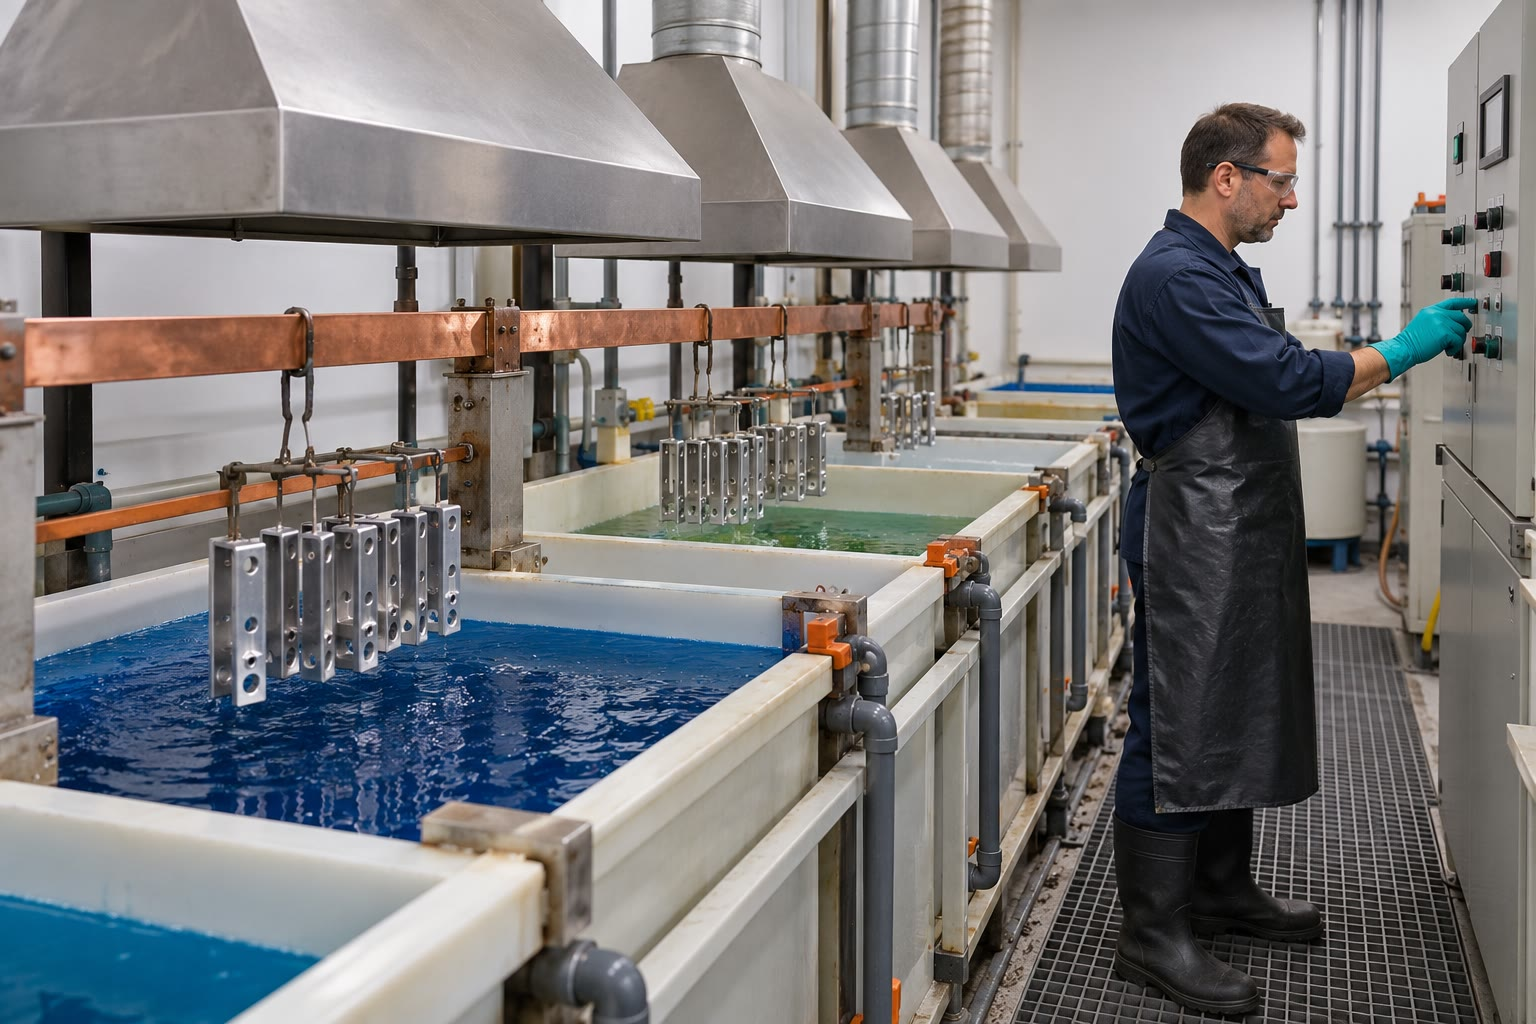
\includegraphics[width=0.62\linewidth]{images/book3/ai/b2-10-electroplating.jpg}

{\small Una línea de galvanizado: las piezas que hay que recubrir cuelgan de barras de cobre
dentro de los baños y actúan como cátodo; el operario ajusta la corriente
en el rectificador. La corriente fija a qué velocidad se deposita el metal; el potencial
de las piezas decide qué metal, o cuánto hidrógeno, se forma con él.}
\end{omfigure}

\section{Un electrodo fuera del equilibrio}

\begin{definition}[Curva intensidad--potencial]\label{def:b2:current-potential-curves:ie-curve}
La \emph{curva intensidad--potencial}\index{curva intensidad--potencial} de un
electrodo en una disolución es la representación de la corriente $i$ que atraviesa el electrodo
en función de su potencial $E$. Una \emph{corriente anódica}\index{corriente anodica@corriente anódica},
contada como positiva, corresponde a una oxidación en el electrodo; una
\emph{corriente catódica}\index{corriente catodica@corriente catódica}, contada como negativa, a una
reducción.
\end{definition}

\begin{definition}[Especie electroactiva]\label{def:b2:current-potential-curves:electroactive}
Una \emph{especie electroactiva}\index{especie electroactiva} es una especie
que puede oxidarse o reducirse en el electrodo en el intervalo de potenciales
considerado.
\end{definition}

\begin{proposition}[Corriente y velocidad]\label{prop:b2:current-potential-curves:current-rate}
Si en un electrodo tiene lugar una sola semirreacción con $n$ electrones, la
corriente mide su velocidad: $i = nF\,d\xi/dt$, siendo $\xi$ el avance de
la oxidación (de modo que $i > 0$ para una oxidación e $i < 0$ para una reducción).
\end{proposition}

\begin{proof}
Por la \cref{prop:b2:cell-thermodynamics:charge}, un avance $d\xi$ hace pasar la
carga $nF\,d\xi$ por el electrodo en el tiempo $dt$.
\end{proof}

Para registrar una curva así, hay que imponer y medir el potencial de un electrodo
mientras circula una corriente por él, cosa que una celda de dos electrodos
no puede hacer, ya que la corriente cambia también el potencial del segundo
electrodo.

\begin{definition}[Montaje de tres electrodos]\label{def:b2:current-potential-curves:set-up}
En un montaje de tres electrodos, la corriente circula entre el \emph{electrodo
de trabajo}\index{electrodo de trabajo}, el que se estudia, y el \emph{contraelectrodo}\index{contraelectrodo},
que cierra el circuito; el potencial
del electrodo de trabajo se mide frente a un electrodo de referencia por el que
no circula corriente. Un potenciostato electrónico ajusta la corriente para
que ese potencial mantenga el valor impuesto.
\end{definition}

\begin{omfigure}
\begin{tikzpicture}[font=\small, >={Stealth}]
  \pic[transform shape] at (0,0) {beaker={0.7}{omDef!14}};
  \pic at (-0.55,0.25) {electrode={black!35}};
  \pic at (0.55,0.25) {electrode={black!15}};
  \pic (r) at (0.0,0.15) {probe};
  \draw[thick, rounded corners] (-2.2,4.3) rectangle (2.2,5.5);
  \node at (0,4.9) {potenciostato};
  \draw[thick, omThm] (-0.40,2.65) -- (-0.40,3.5) -- (-1.6,3.5) -- (-1.6,4.3);
  \draw[thick, omDef] (0.70,2.65) -- (0.70,3.5) -- (1.6,3.5) -- (1.6,4.3);
  \draw[thick] (r-top) -- (0,4.3);
  \node[anchor=east, font=\scriptsize, omThm] at (-1.65,3.85) {ET};
  \node[anchor=west, font=\scriptsize, omDef] at (1.65,3.85) {CE};
  \node[anchor=west, font=\scriptsize] at (0.05,3.95) {ER};
  \draw[<-, omProp, thick] (-0.75,1.2) -- (-2.0,1.4) node[left, text=black, align=right] {electrodo\\ de trabajo};
  \draw[<-, omProp, thick] (0.85,1.2) -- (2.1,1.4) node[right, text=black, align=left] {contra-\\ electrodo};
  \draw[<-, omProp, thick] (0.05,0.5) -- (1.4,-0.4) node[right, text=black] {electrodo de referencia};
  \node[font=\scriptsize, align=center] at (0,6.0) {impone $E_{\text{ET}} - E_{\text{ER}}$, mide $i$};
\end{tikzpicture}

{\small El montaje de tres electrodos. El potenciostato hace circular la corriente
entre el \omterm{def:b2:current-potential-curves:set-up}{electrodo de trabajo} (ET) y el \omterm{def:b2:current-potential-curves:set-up}{contraelectrodo} (CE) de modo que
mantiene el potencial del \omterm{def:b2:current-potential-curves:set-up}{electrodo de trabajo}, medido frente al electrodo de
referencia (ER), en el valor impuesto; por el electrodo de referencia no circula
corriente.}
\end{omfigure}

Cuando no circula corriente y están presentes las dos formas de un par, el electrodo
toma el potencial de Nernst del par, si el intercambio de electrones es lo bastante rápido
para establecerlo. Alejar el potencial de ese valor hace circular una
corriente.

\section{Sistemas rápidos y lentos}

\begin{definition}[Sobretensión]\label{def:b2:current-potential-curves:overpotential}
La \emph{sobretensión}\index{sobretension@sobretensión} de un electrodo por el que circula una
corriente $i$ es $\eta = E(i) - E_{\text{eq}}$, la diferencia entre su
potencial y el potencial de equilibrio (de Nernst) del par. El
\emph{potencial umbral}\index{potencial umbral} de una semirreacción es el
potencial a partir del cual su corriente se vuelve apreciable.
\end{definition}

\begin{definition}[Sistemas rápidos y lentos]\label{def:b2:current-potential-curves:fast-slow}
Un par es un \emph{sistema rápido}\index{sistema rapido@sistema rápido} en un electrodo dado si
circula una corriente apreciable en cuanto el potencial se aleja de su potencial de
Nernst; es un \emph{sistema lento}\index{sistema lento} si hace falta una \omterm{def:b2:current-potential-curves:overpotential}{sobretensión} de
algunas décimas de voltio para que la corriente sea apreciable, en
uno u otro sentido.
\end{definition}

Que un sistema sea rápido o lento depende del par y del material del
electrodo. Los pares \ce{Fe^3+}/\ce{Fe^2+} y \ce{Ag+}/\ce{Ag} son rápidos sobre
platino; la reducción de \ce{H+} es rápida sobre platino pero lenta sobre mercurio,
plomo o cinc; la oxidación del agua a dioxígeno es lenta sobre cualquier electrodo.
Las transferencias de electrones que rompen o forman enlaces, como las de \ce{O2} o \ce{H2},
suelen ser lentas; la transferencia de un electrón entre dos iones de forma casi
igual es rápida. La forma de la parte ascendente de una curva lenta procede de
la cinética de la transferencia electrónica, que se deduce en el volumen del tercer año.

\begin{omfigure}
\begin{tikzpicture}
\begin{axis}[omie, width=0.47\linewidth, height=5.4cm, xmin=0.25, xmax=1.3,
  ymin=-1.3, ymax=1.3, xlabel={$E$}, ylabel={$i$}, title={\small sistema rápido}]
\addplot[omanodic] table[x=E, y=i, restrict expr to domain={\thisrow{i}}{0:2}] {figdata/out/bachelor-2-ie-curves-a.dat};
\addplot[omcathodic] table[x=E, y=i, restrict expr to domain={\thisrow{i}}{-2:0}] {figdata/out/bachelor-2-ie-curves-a.dat};
\draw[densely dotted] (axis cs:0.77,-1.2) -- (axis cs:0.77,1.2);
\node[font=\scriptsize, anchor=north west] at (axis cs:0.78,-0.05) {$E_{\text{eq}}$};
\node[font=\scriptsize, anchor=south] at (axis cs:1.1,1.0) {\ce{Fe^2+} $\to$ \ce{Fe^3+}};
\node[font=\scriptsize, anchor=north] at (axis cs:0.45,-1.0) {\ce{Fe^3+} $\to$ \ce{Fe^2+}};
\end{axis}
\end{tikzpicture}\hfill
\begin{tikzpicture}
\begin{axis}[omie, width=0.47\linewidth, height=5.4cm, xmin=-0.25, xmax=1.8,
  ymin=-1.3, ymax=1.3, xlabel={$E$}, ylabel={$i$}, title={\small sistema lento}]
\addplot[omanodic] table[x=E, y=i, restrict expr to domain={\thisrow{i}}{0:2}] {figdata/out/bachelor-2-ie-curves-c.dat};
\addplot[omcathodic] table[x=E, y=i, restrict expr to domain={\thisrow{i}}{-2:0}] {figdata/out/bachelor-2-ie-curves-c.dat};
\draw[densely dotted] (axis cs:0.77,-1.2) -- (axis cs:0.77,1.2);
\draw[<->, omProp] (axis cs:0.77,0.5) -- (axis cs:1.12,0.5) node[midway, above, font=\scriptsize] {$\eta_a$};
\draw[<->, omProp] (axis cs:0.42,-0.5) -- (axis cs:0.77,-0.5) node[midway, below, font=\scriptsize] {$\eta_c$};
\node[font=\scriptsize, anchor=north west] at (axis cs:0.78,-0.05) {$E_{\text{eq}}$};
\end{axis}
\end{tikzpicture}

{\small \omterm{def:b2:current-potential-curves:ie-curve}{Curvas intensidad--potencial} modelo de un par cuyas dos formas están presentes
a concentraciones iguales (rama anódica en rojo, catódica en azul). A la izquierda, un \omterm{def:b2:current-potential-curves:fast-slow}{sistema
rápido}: la corriente cambia de signo bruscamente en el potencial de equilibrio. A la derecha,
un \omterm{def:b2:current-potential-curves:fast-slow}{sistema lento}: no circula corriente en un intervalo de potenciales a su alrededor; cada
rama necesita una \omterm{def:b2:current-potential-curves:overpotential}{sobretensión}. Ambas alcanzan las mismas mesetas límite, fijadas por la
difusión. (Valores ilustrativos.)}
\end{omfigure}

\section{Transporte de materia y corrientes límite}

Cuando la transferencia electrónica es rápida, la corriente está limitada por la llegada del
reactivo al electrodo. En una disolución agitada, una fina capa de líquido
junto al electrodo permanece casi inmóvil, y el reactivo la atraviesa por
difusión.

\begin{definition}[Capa de difusión y corriente límite]\label{def:b2:current-potential-curves:limiting-current}
La \emph{capa de difusión}\index{capa de difusion@capa de difusión} es la capa de disolución,
de espesor $\delta$ (de unos pocos a algunas decenas de micrómetros en una disolución
agitada), junto al electrodo, a través de la cual las especies se desplazan solo por
difusión. La \emph{corriente límite}\index{corriente limite@corriente límite} es la corriente
que se alcanza cuando la \omterm{def:b2:current-potential-curves:electroactive}{especie electroactiva} se consume tan deprisa como llega, siendo
nula su concentración en la superficie.
\end{definition}

\begin{omfigure}
\begin{tikzpicture}[font=\small, >={Stealth}, x=1.2cm, y=1.2cm]
  \fill[black!25] (-0.4,0) rectangle (0,3);
  \node[rotate=90, font=\scriptsize] at (-0.2,1.5) {electrodo};
  \draw[->] (0,0) -- (4.6,0) node[right] {$x$};
  \draw[->] (0,0) -- (0,3.2) node[above] {$c$};
  \draw[densely dashed] (1.6,0) -- (1.6,3);
  \node[below, font=\scriptsize] at (1.6,0) {$\delta$};
  \draw[omDef, thick] (0,1.2) -- (1.6,2.4) -- (4.4,2.4);
  \draw[omThm, thick] (0,0.02) -- (1.6,2.4);
  \node[font=\scriptsize, anchor=west] at (2.6,2.6) {seno, $c^b$ (agitado)};
  \node[font=\scriptsize, omDef, anchor=east] at (-0.45,1.2) {$c^s$};
  \node[font=\scriptsize, omThm, anchor=west] at (1.7,0.5) {$c^s = 0$: corriente límite};
  \node[font=\scriptsize, align=center] at (0.8,3.0) {capa de\\ difusión};
\end{tikzpicture}

{\small Concentración del reactivo cerca de un electrodo en una disolución
agitada. A través de la \omterm{def:b2:current-potential-curves:limiting-current}{capa de difusión} el perfil es lineal; el flujo, y con él la
corriente, es proporcional a $c^b - c^s$. Es máximo cuando el reactivo se
consume en cuanto llega ($c^s = 0$, rojo).}
\end{omfigure}

\begin{theorem}[Corriente límite]\label{thm:b2:current-potential-curves:limiting}
Para una especie de concentración $c$ en el seno de la disolución y coeficiente de difusión $D$,
que atraviesa una \omterm{def:b2:current-potential-curves:limiting-current}{capa de difusión} de espesor $\delta$ hasta un electrodo de área $A$,
la \omterm{def:b2:current-potential-curves:limiting-current}{corriente límite} es, en valor absoluto,
\[
  |i_{\lim}| = \frac{nFADc}{\delta} .
\]
\end{theorem}

\begin{proof}
En régimen estacionario el perfil de concentración en la capa es lineal (la segunda ley
de Fick con $\partial c/\partial t = 0$ da $d^2c/dx^2 = 0$), de modo que el flujo
hacia el electrodo es $j = D(c - c^s)/\delta$, en moles por unidad de área y de
tiempo. Cada molécula que llega reacciona con $n$ electrones: $|i| = nFAj =
nFAD(c - c^s)/\delta$, máxima para $c^s = 0$.
\end{proof}

\begin{example}[Orden de magnitud de una corriente límite]\label{ex:b2:current-potential-curves:ilim}
Para una especie a \qty{10}{mmol/L} (\qty{10}{mol/m^3}), con $D =
\qty{7e-10}{m^2/s}$, $\delta = \qty{20}{\micro m}$, $n = 1$, sobre
\qty{1.0}{cm^2}: $|i_{\lim}| = 96\,485 \times 10^{-4} \times 7 \times 10^{-10}
\times 10/(2 \times 10^{-5}) = \qty{3.4}{mA}$.
\end{example}

\begin{theorem}[Onda de un sistema rápido]\label{thm:b2:current-potential-curves:wave}
Para un par rápido $\mathrm{Ox} + n\,\mathrm e^- \rightleftharpoons \mathrm{Red}$,
con \omterm{def:b2:current-potential-curves:limiting-current}{corriente límite} anódica $i_{\lim,a} > 0$ (fijada por Red) y \omterm{def:b2:current-potential-curves:limiting-current}{corriente límite}
catódica $i_{\lim,c} < 0$ (fijada por Ox), la curva en régimen estacionario es
\[
  E = E_{1/2} + \frac{RT}{nF}\ln\frac{i - i_{\lim,c}}{i_{\lim,a} - i},
  \qquad E_{1/2} = E^\circ + \frac{RT}{nF}\ln\frac{D_{\text{Red}}}{D_{\text{Ox}}} ,
\]
siendo el espesor de la capa el mismo para ambas formas.
\end{theorem}

\begin{proof}
\omterm{def:b2:current-potential-curves:fast-slow}{Sistema rápido}: la ecuación de Nernst se cumple en la superficie, $E = E^\circ + (RT/nF)
\ln(c^s_{\text{Ox}}/c^s_{\text{Red}})$. Perfiles lineales: una \omterm{def:b2:current-potential-curves:ie-curve}{corriente anódica} $i$
consume Red y produce Ox en la superficie, $i = nFAD_{\text{Red}}(c^b_{\text{Red}}
- c^s_{\text{Red}})/\delta = -nFAD_{\text{Ox}}(c^b_{\text{Ox}} - c^s_{\text{Ox}})/\delta$.
Con $i_{\lim,a} = nFAD_{\text{Red}}c^b_{\text{Red}}/\delta$ e $i_{\lim,c} =
-nFAD_{\text{Ox}}c^b_{\text{Ox}}/\delta$, se obtiene $c^s_{\text{Red}} = (i_{\lim,a} -
i)\delta/(nFAD_{\text{Red}})$ y $c^s_{\text{Ox}} = (i - i_{\lim,c})\delta/(nFAD_{\text{Ox}})$.
Se sustituye en la ecuación de Nernst.
\end{proof}

\begin{corollary}[Potencial de semionda]\label{cor:b2:current-potential-curves:half-wave}
Cuando las dos formas tienen coeficientes de difusión iguales, $E_{1/2} = E^\circ$: con
una sola forma presente, la corriente vale la mitad de su valor límite en el potencial
estándar del par.
\end{corollary}

\begin{proof}
Con solo Red presente, $i_{\lim,c} = 0$, y para $i = i_{\lim,a}/2$ el logaritmo
se anula: $E = E_{1/2} = E^\circ$ cuando $D_{\text{Red}} = D_{\text{Ox}}$.
\end{proof}

\begin{proposition}[Las mesetas miden concentraciones]\label{prop:b2:current-potential-curves:plateau}
Con agitación y electrodo fijos, la altura de una meseta es proporcional a la
concentración de la especie que consume: un electrodo mantenido a un
potencial de la meseta es un sensor amperométrico.
\end{proposition}

\begin{proof}
$|i_{\lim}| = (nFAD/\delta)\,c$, y el factor entre paréntesis es constante con agitación
y temperatura fijas.
\end{proof}

\begin{omfigure}
\begin{tikzpicture}
\begin{axis}[omie, width=0.47\linewidth, height=5.0cm, xmin=0.25, xmax=1.3,
  ymin=-0.3, ymax=1.3, xlabel={$E$}, ylabel={$i$}, title={\small solo \ce{Fe^2+} presente}]
\addplot[omanodic] table[x=E, y=i] {figdata/out/bachelor-2-ie-curves-b.dat};
\draw[densely dotted] (axis cs:0.77,0) -- (axis cs:0.77,0.5) -- (axis cs:0.25,0.5);
\node[font=\scriptsize, anchor=north] at (axis cs:0.77,-0.02) {$E_{1/2}$};
\node[font=\scriptsize, anchor=south west] at (axis cs:0.27,0.5) {$i_{\lim}/2$};
\node[font=\scriptsize, anchor=south] at (axis cs:1.12,1.0) {meseta};
\end{axis}
\end{tikzpicture}\hfill
\begin{tikzpicture}
\begin{axis}[width=0.42\linewidth, height=5.0cm, xmin=0, xmax=1.05, ymin=0, ymax=1.1,
  axis x line=bottom, axis y line=left, xtick=\empty, ytick=\empty,
  xlabel={$c$}, ylabel={$i_{\lim}$}, label style={font=\small},
  title={\small amperometría}]
\addplot[omanodic, mark=*, mark size=1.2pt] table[x=c, y=i] {figdata/out/bachelor-2-ie-curves-e.dat};
\end{axis}
\end{tikzpicture}

{\small A la izquierda: la onda de un par rápido cuando solo está presente la forma reducida
(modelo); su altura mitad está en el potencial de semionda. A la derecha: la altura de la
meseta crece proporcionalmente a la concentración.}
\end{omfigure}

\section{El disolvente y el electrodo}

El agua misma es electroactiva: se oxida a dioxígeno
(\ce{2H2O -> O2 + 4H+ + 4e-}) y se reduce a dihidrógeno (\ce{2H+ + 2e- -> H2}, o
\ce{2H2O + 2e- -> H2 + 2OH-}). Como el disolvente nunca se agota, sus curvas
no tienen meseta: suben bruscamente y acotan todas las demás curvas.

\begin{definition}[Ventana de electroactividad]\label{def:b2:current-potential-curves:window}
Los \emph{muros del disolvente}\index{muro del disolvente} son las ramas abruptas de la
oxidación y la reducción del disolvente. La \emph{ventana de
electroactividad}\index{ventana de electroactividad} es el intervalo de potenciales comprendido entre ellos,
en el que pueden observarse las curvas de las especies disueltas.
\end{definition}

\begin{proposition}[La ventana del agua]\label{prop:b2:current-potential-curves:window}
En agua a un pH dado, la ventana se sitúa en torno al intervalo termodinámico de los
dos pares del agua, $\qty{0}{V} - 0.059\,\mathrm{pH}$ y $\qty{1.23}{V} -
0.059\,\mathrm{pH}$, ensanchado a cada lado por la \omterm{def:b2:current-potential-curves:overpotential}{sobretensión} de la
reacción correspondiente sobre el electrodo empleado.
\end{proposition}

\begin{proof}[Argumento]
Cada muro empieza cerca del potencial de Nernst de su par desplazado por la
\omterm{def:b2:current-potential-curves:overpotential}{sobretensión} umbral: la oxidación del agua es lenta sobre todos los electrodos, así que
el muro anódico está algunas décimas de voltio por encima de \qty{1.23}{V} (a pH 0); la
reducción de \ce{H+} es rápida sobre platino, cuyo muro catódico queda cerca de
\qty{0}{V}, pero lenta sobre cinc, plomo o mercurio, cuyo muro está varias décimas de
voltio más abajo.
\end{proof}

\begin{omfigure}
\begin{tikzpicture}
\begin{axis}[omie, width=0.82\linewidth, height=5.4cm, xmin=-1.2, xmax=2.0,
  ymin=-3, ymax=3, xlabel={$E$ (V)}, ylabel={$i$}, clip=true, clip mode=individual]
\addplot[omwall] table[x=E, y=i] {figdata/out/bachelor-2-ie-curves-d-high.dat};
\addplot[omcathodic] table[x=E, y=i, restrict expr to domain={\thisrow{E}}{-1.2:0.6}] {figdata/out/bachelor-2-ie-curves-d-Pt.dat};
\addplot[omanodic] table[x=E, y=i, restrict expr to domain={\thisrow{E}}{0.6:2.0}] {figdata/out/bachelor-2-ie-curves-d-Pt.dat};
\draw[densely dotted] (axis cs:0,-2.8) -- (axis cs:0,2.8);
\draw[densely dotted] (axis cs:1.23,-2.8) -- (axis cs:1.23,2.8);
\node[font=\scriptsize, anchor=north west] at (axis cs:0.02,-0.1) {0};
\node[font=\scriptsize, anchor=north west] at (axis cs:1.24,-0.1) {1.23};
\node[font=\scriptsize, omDef, anchor=west] at (axis cs:0.05,-2.2) {\ce{H+} $\to$ \ce{H2} sobre Pt};
\node[font=\scriptsize, gray, anchor=east] at (axis cs:-0.85,-1.0) {sobre Zn, Pb};
\node[font=\scriptsize, omThm, anchor=east] at (axis cs:1.18,2.2) {\ce{H2O} $\to$ \ce{O2}};
\end{axis}
\end{tikzpicture}

{\small Los muros del agua a pH 0 (modelo). La reducción de \ce{H+} empieza cerca de
\qty{0}{V} sobre platino (azul), pero varias décimas de voltio más abajo sobre metales como
el cinc o el plomo (discontinua); la oxidación del agua necesita una \omterm{def:b2:current-potential-curves:overpotential}{sobretensión} sobre cualquier
electrodo. La ventana es el intervalo entre los muros.}
\end{omfigure}

\section{Lectura de las curvas}

\begin{method}[Esbozar las curvas de una disolución]\label{met:b2:current-potential-curves:sketch-ie}
\begin{enumerate}
  \item Trácense los dos \omterm{def:b2:current-potential-curves:window}{muros del disolvente} para el pH y el material del
        electrodo.
  \item Para cada par presente, sitúese su potencial de Nernst (ambas formas
        presentes) o $E^\circ$ (una sola forma): un \omterm{def:b2:current-potential-curves:fast-slow}{sistema rápido} corta el eje ahí
        bruscamente; un \omterm{def:b2:current-potential-curves:fast-slow}{sistema lento} queda desplazado por sus \omterm{def:b2:current-potential-curves:overpotential}{sobretensiones}.
  \item Dese a cada onda una meseta proporcional a la concentración de la
        especie que consume; un electrodo metálico que se oxida a sí mismo no tiene
        meseta (el metal no se agota).
  \item Súmense las corrientes de las reacciones posibles a cada potencial.
\end{enumerate}
\end{method}

\begin{method}[Leer las curvas]\label{met:b2:current-potential-curves:read-ie}
\begin{enumerate}
  \item A un potencial impuesto, léase en cada curva la corriente de cada
        reacción: transcurren simultáneamente, en proporción a sus corrientes.
  \item A una corriente impuesta (electrólisis), búsquese el potencial al que las
        curvas anódicas o catódicas suman esa corriente; las reacciones que
        intervienen son aquellas cuyas curvas contribuyen allí.
  \item Para una pila, o un metal que se corroe, la \omterm{def:b2:current-potential-curves:ie-curve}{corriente anódica} de una reacción
        es igual a la \omterm{def:b2:current-potential-curves:ie-curve}{corriente catódica} de la otra: búsquese ese par de
        puntos.
\end{enumerate}
\end{method}

\begin{example}[Cincado a partir de un baño ácido]\label{ex:b2:current-potential-curves:zinc}
En un baño ácido de cinc, el cátodo admite dos reducciones posibles: \ce{Zn^2+
+ 2e- -> Zn} ($E^\circ = \qty{-0.76}{V}$, rápida) y \ce{2H+ + 2e- -> H2}
($E^\circ = \qty{0}{V}$). Termodinámicamente, el hidrógeno debería formarse primero y el cinc
nunca. Pero sobre cinc la reducción de \ce{H+} es lenta: su muro está por debajo de
\qty{-0.76}{V}, y al potencial al que el cinc se deposita a una velocidad
útil se forma poco hidrógeno. La curva, no el diagrama, explica el
recubrimiento.
\end{example}

\begin{history}[Polarografía]
\begin{minipage}[t]{0.25\linewidth}
\vspace{0pt}
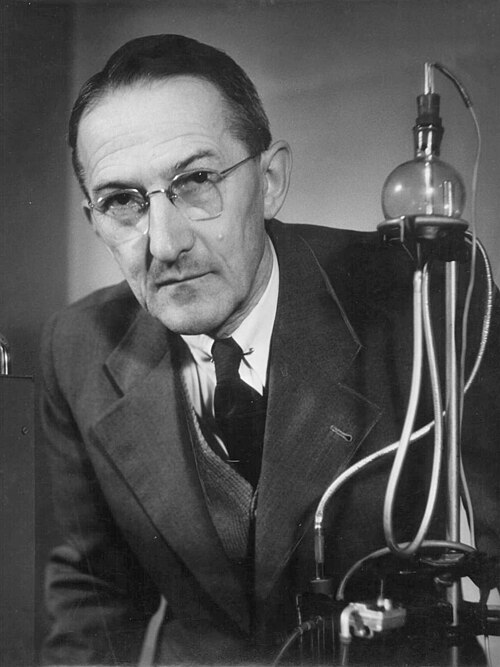
\includegraphics[width=\linewidth]{images/book3/heyrovsky.jpg}
\end{minipage}\hfill
\begin{minipage}[t]{0.71\linewidth}
\vspace{0pt}
En 1922 Jaroslav Heyrovský registró la corriente a través de un electrodo de mercurio
que se formaba gota a gota en la punta de un capilar, mientras se barría el potencial:
cada especie reducible daba un escalón cuya posición la identificaba y
cuya altura medía su concentración. La gota renovada mantenía la superficie
limpia, y la elevada \omterm{def:b2:current-potential-curves:overpotential}{sobretensión} del hidrógeno sobre el mercurio abría una amplia
ventana catódica. La polarografía le valió el Premio Nobel de Química en 1959
y fundó la química electroanalítica; la fotografía lo muestra con un
electrodo de gota de mercurio. (Fotografía: archivo del Instituto J.~Heyrovský
de Química Física, CC BY-SA 3.0, Wikimedia Commons.)
\end{minipage}
\end{history}

\section{Ejercicios}

\begin{exercise}[$\star$]\label{exo:b2:current-potential-curves:1}
En una pila Daniell que suministra corriente, dese el signo de la corriente en el
electrodo de cinc y en el electrodo de cobre, con los convenios de este
capítulo.
\end{exercise}

\begin{exercise}[$\star$]\label{exo:b2:current-potential-curves:2}
Calcúlese la \omterm{def:b2:current-potential-curves:limiting-current}{corriente límite} de la reducción de \ce{Ag+} (\qty{2.0}{mmol/L}, $D =
\qty{1.6e-9}{m^2/s}$) sobre \qty{0.50}{cm^2} con $\delta = \qty{25}{\micro m}$
(valores del modelo).
\end{exercise}

\begin{exercise}[$\star$]\label{exo:b2:current-potential-curves:3}
En las curvas modelo del capítulo, ¿cómo se reconoce un \omterm{def:b2:current-potential-curves:fast-slow}{sistema rápido} y uno
lento? Dese un ejemplo de cada uno sobre platino.
\end{exercise}

\begin{exercise}[$\star$]\label{exo:b2:current-potential-curves:4}
Una disolución contiene solo \ce{Fe^2+}. ¿A qué potencial alcanza su \omterm{def:b2:current-potential-curves:ie-curve}{corriente anódica}
la mitad de su meseta, si las dos formas difunden igual ($E^\circ = \qty{0.77}{V}$)?
\end{exercise}

\begin{exercise}[$\star\star$]\label{exo:b2:current-potential-curves:5}
Un electrodo de platino en una disolución de \ce{Fe^3+} y \ce{Cu^2+} (concentraciones
iguales, $E^\circ$ = 0.77 y \qty{0.34}{V}) se barre hacia potenciales
negativos. Descríbase la curva: ondas, mesetas, sus alturas y el muro
catódico.
\end{exercise}

\begin{exercise}[$\star\star$]\label{exo:b2:current-potential-curves:6}
En la disolución del \cref{exo:b2:current-potential-curves:5}, el potencial del
electrodo se mantiene en \qty{0.50}{V} y luego en \qty{0.10}{V}. ¿Qué ocurre en
cada caso?
\end{exercise}

\begin{exercise}[$\star\star$]\label{exo:b2:current-potential-curves:7}
Dense los potenciales de Nernst de los dos pares del agua a pH 0 y a pH 14, y
esbócese cómo se desplaza con el pH la ventana sobre platino.
\end{exercise}

\begin{exercise}[$\star\star$]\label{exo:b2:current-potential-curves:8}
Se valora \ce{Fe^2+} con \ce{Ce^4+} mientras un electrodo de platino mantenido a
\qty{1.0}{V} registra la corriente. Esbócese la corriente en función del volumen añadido
y explíquese cómo localiza la equivalencia (\ce{Ce^4+}/\ce{Ce^3+}: $E^\circ =
\qty{1.72}{V}$).
\end{exercise}

\begin{exercise}[$\star\star$]\label{exo:b2:current-potential-curves:9}
Duplicar la velocidad de agitación reduce a la mitad el espesor de la \omterm{def:b2:current-potential-curves:limiting-current}{capa de difusión}. ¿Qué
les ocurre a las mesetas, al potencial de semionda y al potencial de corriente
nula de un \omterm{def:b2:current-potential-curves:fast-slow}{sistema rápido}?
\end{exercise}

\begin{exercise}[$\star\star\star$]\label{exo:b2:current-potential-curves:10}
Dedúzcase la ecuación de la onda de un \omterm{def:b2:current-potential-curves:fast-slow}{sistema rápido} con solo Red presente, y
demuéstrese que una representación de $E$ frente a $\log[i/(i_{\lim} - i)]$ es una recta de
pendiente $0.059/n$ voltios a \qty{25}{\degreeCelsius}.
\end{exercise}

\begin{exercise}[$\star\star\star$]\label{exo:b2:current-potential-curves:11}
Un trozo de cinc sumergido en ácido de \qty{1}{mol/L} se disuelve solo lentamente, mientras que
el mismo trozo en contacto con un hilo de platino se disuelve deprisa, con hidrógeno burbujeando
sobre el platino. Explíquese con \omterm{def:b2:current-potential-curves:ie-curve}{curvas intensidad--potencial}.
\end{exercise}

\begin{exercise}[$\star\star\star$]\label{exo:b2:current-potential-curves:12}
Para oxidar una especie cuya onda está a \qty{2.0}{V} a pH 0, ¿se elegiría un
electrodo de platino o uno con una \omterm{def:b2:current-potential-curves:overpotential}{sobretensión} de oxígeno elevada? Explíquese, y dígase
qué se formaría en otro caso.
\end{exercise}

\section{Problema: una sonda de oxígeno para un río}

\begin{problem}[{Problema de fin de semana --- el cátodo de un sensor amperométrico de
oxígeno, la corriente límite a través de su membrana, la calibración en
agua saturada de aire con la ley de Henry y el contenido de oxígeno de un río}]
\label{pb:b2:current-potential-curves:1}
Una sonda amperométrica de oxígeno tiene un cátodo de oro y un ánodo de plata en un
gel de cloruro de potasio, separados de la muestra por una fina membrana permeable
a los gases. El cátodo se mantiene a \qty{-0.60}{V} frente al ánodo de plata--cloruro
de plata. Datos a \qty{25}{\degreeCelsius}: constante de la \omterm{prop:b2:chemical-potential:henry}{ley de Henry} del
\ce{O2}, $H = \qty{1.3e-5}{mol/(m^3.Pa)}$; presión de vapor del agua
\qty{3.17}{kPa}; oxígeno en el aire seco, 20.95~\% en volumen; $E^\circ(\ce{O2}/\ce{H2O}) =
\qty{1.229}{V}$; $E^\circ(\ce{AgCl}/\ce{Ag}) = \qty{0.222}{V}$. Membrana (valores del
modelo): área \qty{0.10}{cm^2}, espesor \qty{25}{\micro m}, coeficiente de difusión
efectivo del \ce{O2} a su través \qty{1.0e-10}{m^2/s}.
% ledger: henry:O2, pvap:H2O.298, air:O2, dfg:Cl-_ao, dfg:AgCl_cr, aw:O

\medskip
\noindent\textbf{Parte I --- El cátodo.}
\begin{enumerate}
  \item Escríbase la reducción del dioxígeno en medio neutro.
  \item Escríbanse la reacción en el ánodo de plata y la reacción global.
  \item Calcúlese el potencial de Nernst del par \ce{O2}/\ce{H2O} a pH 7 con
        $p_{\ce{O2}} = \qty{0.21}{bar}$.
  \item Exprésese el potencial del cátodo, \qty{-0.60}{V} frente a Ag/AgCl, en la
        escala del hidrógeno, tomando como 1 la actividad del cloruro del gel.
  \item ¿Por qué debe mantenerse el cátodo muy por debajo del potencial de Nernst del
        \ce{O2}?
  \item ¿Por qué se elige un potencial situado en la meseta?
  \item ¿Qué fija el límite inferior de los potenciales utilizables?
\end{enumerate}

\medskip
\noindent\textbf{Parte II --- La \omterm{def:b2:current-potential-curves:limiting-current}{corriente límite}.}
\begin{enumerate}[resume]
  \item Descríbase el perfil de concentración del \ce{O2} a través de la membrana cuando el
        cátodo trabaja en su meseta.
  \item Escríbase el flujo de \ce{O2} a través de la membrana.
  \item Dedúzcase la corriente en función de la concentración $c$ de \ce{O2}
        disuelto.
  \item ¿Por qué se usa el espesor de la membrana en lugar de la \omterm{def:b2:current-potential-curves:limiting-current}{capa de difusión}?
  \item ¿Por qué la lectura depende poco de la agitación del río, pero mucho
        del ensuciamiento de la membrana?
\end{enumerate}

\medskip
\noindent\textbf{Parte III --- La calibración.}
\begin{enumerate}[resume]
  \item Calcúlese la presión parcial del \ce{O2} sobre agua saturada de aire a
        \qty{1.013}{bar} y \qty{25}{\degreeCelsius}.
  \item Calcúlese la concentración de \ce{O2} disuelto en la saturación, en
        \unit{mol/m^3}.
  \item Exprésese en \unit{mg/L}.
  \item Predígase la corriente de la sonda en agua saturada de aire.
  \item La sonda marca en realidad \qty{4.05}{\micro A} en agua saturada de aire
        (datos del ejercicio). Calcúlese su sensibilidad en \unit{\micro A} por
        \unit{mg/L}.
  \item ¿Por qué calibrar en lugar de fiarse de la corriente predicha?
  \item ¿Qué debería marcar la sonda en agua desprovista de oxígeno?
\end{enumerate}

\medskip
\noindent\textbf{Parte IV --- El río.}
\begin{enumerate}[resume]
  \item En una muestra de río a \qty{25}{\degreeCelsius}, la sonda marca
        \qty{2.80}{\micro A}. Calcúlese el oxígeno disuelto en \unit{mg/L}.
  \item Exprésese como porcentaje de la saturación.
  \item El agua de un río está casi saturada de oxígeno en su nacimiento.
        Propóngase una causa para el déficit.
  \item ¿Qué cantidad de \ce{O2} consume la sonda en una hora? ¿Perturba la
        muestra?
  \item ¿Por qué debe repetirse la calibración si el río está a
        \qty{15}{\degreeCelsius}?
  \item Indíquese la concentración de oxígeno disuelto de la muestra.
\end{enumerate}
\end{problem}
